\documentclass[11p]{article}
% Packages
\usepackage{amsmath}
\usepackage{graphicx}
\usepackage[swedish]{babel}
\usepackage[
    backend=biber,
    style=authoryear-ibid,
    sorting=ynt
]{biblatex}
\usepackage[utf8]{inputenc}
\usepackage[T1]{fontenc}
\usepackage{blindtext}
\usepackage{siunitx}
\usepackage{enumerate}
%Källor

\graphicspath{ {./images/} }

\title{Labrapprt \\ \small Fysik 1}
\author{Magnus Silverdal }
\date{\today}

\begin{document}

    \begin{titlepage}
        \begin{center}
            \vspace*{1cm}

            \Huge
            \textbf{Laboration 5}

            \vspace{0.5cm}
            \LARGE
            Ellära

            \vspace{1.5cm}

            \textbf{Linus Lundqvist}

            \vfill


            Fysik 1

            \vspace{0.8cm}

            
\includegraphics[width=0.4\textwidth]{NTI Gymnasiet_Symbol_print_svart.png}

            \Large
            Teknikprogrammet\\
            NTI Gymnasiet\\
            Umeå\\
            \today

        \end{center}
    \end{titlepage}
    \section{Syfte och frågeställning}

    Syftet med laborationen var att undersöka Serie- och Parallelkopplingar praktiskt och sedan jämföra med teorin.

    \section{Material}

    \begin{itemize}
        \item 1 - Batteri
        \item 1 - Multimeter
        \item 5 - kablar
        \item 2 - kopplingssplint
        \item 2 - Resistor, $100\Omega$
    \end{itemize}

    \section{Del 1}
    \subsection{Metod}
    Målet med första delen är att bestämma en resistorns resistans.

    \begin{enumerate}
        \item Koppla ihop Batteriet med resistorn.
        \item Koppla multimetern över resistorn.
        \\
        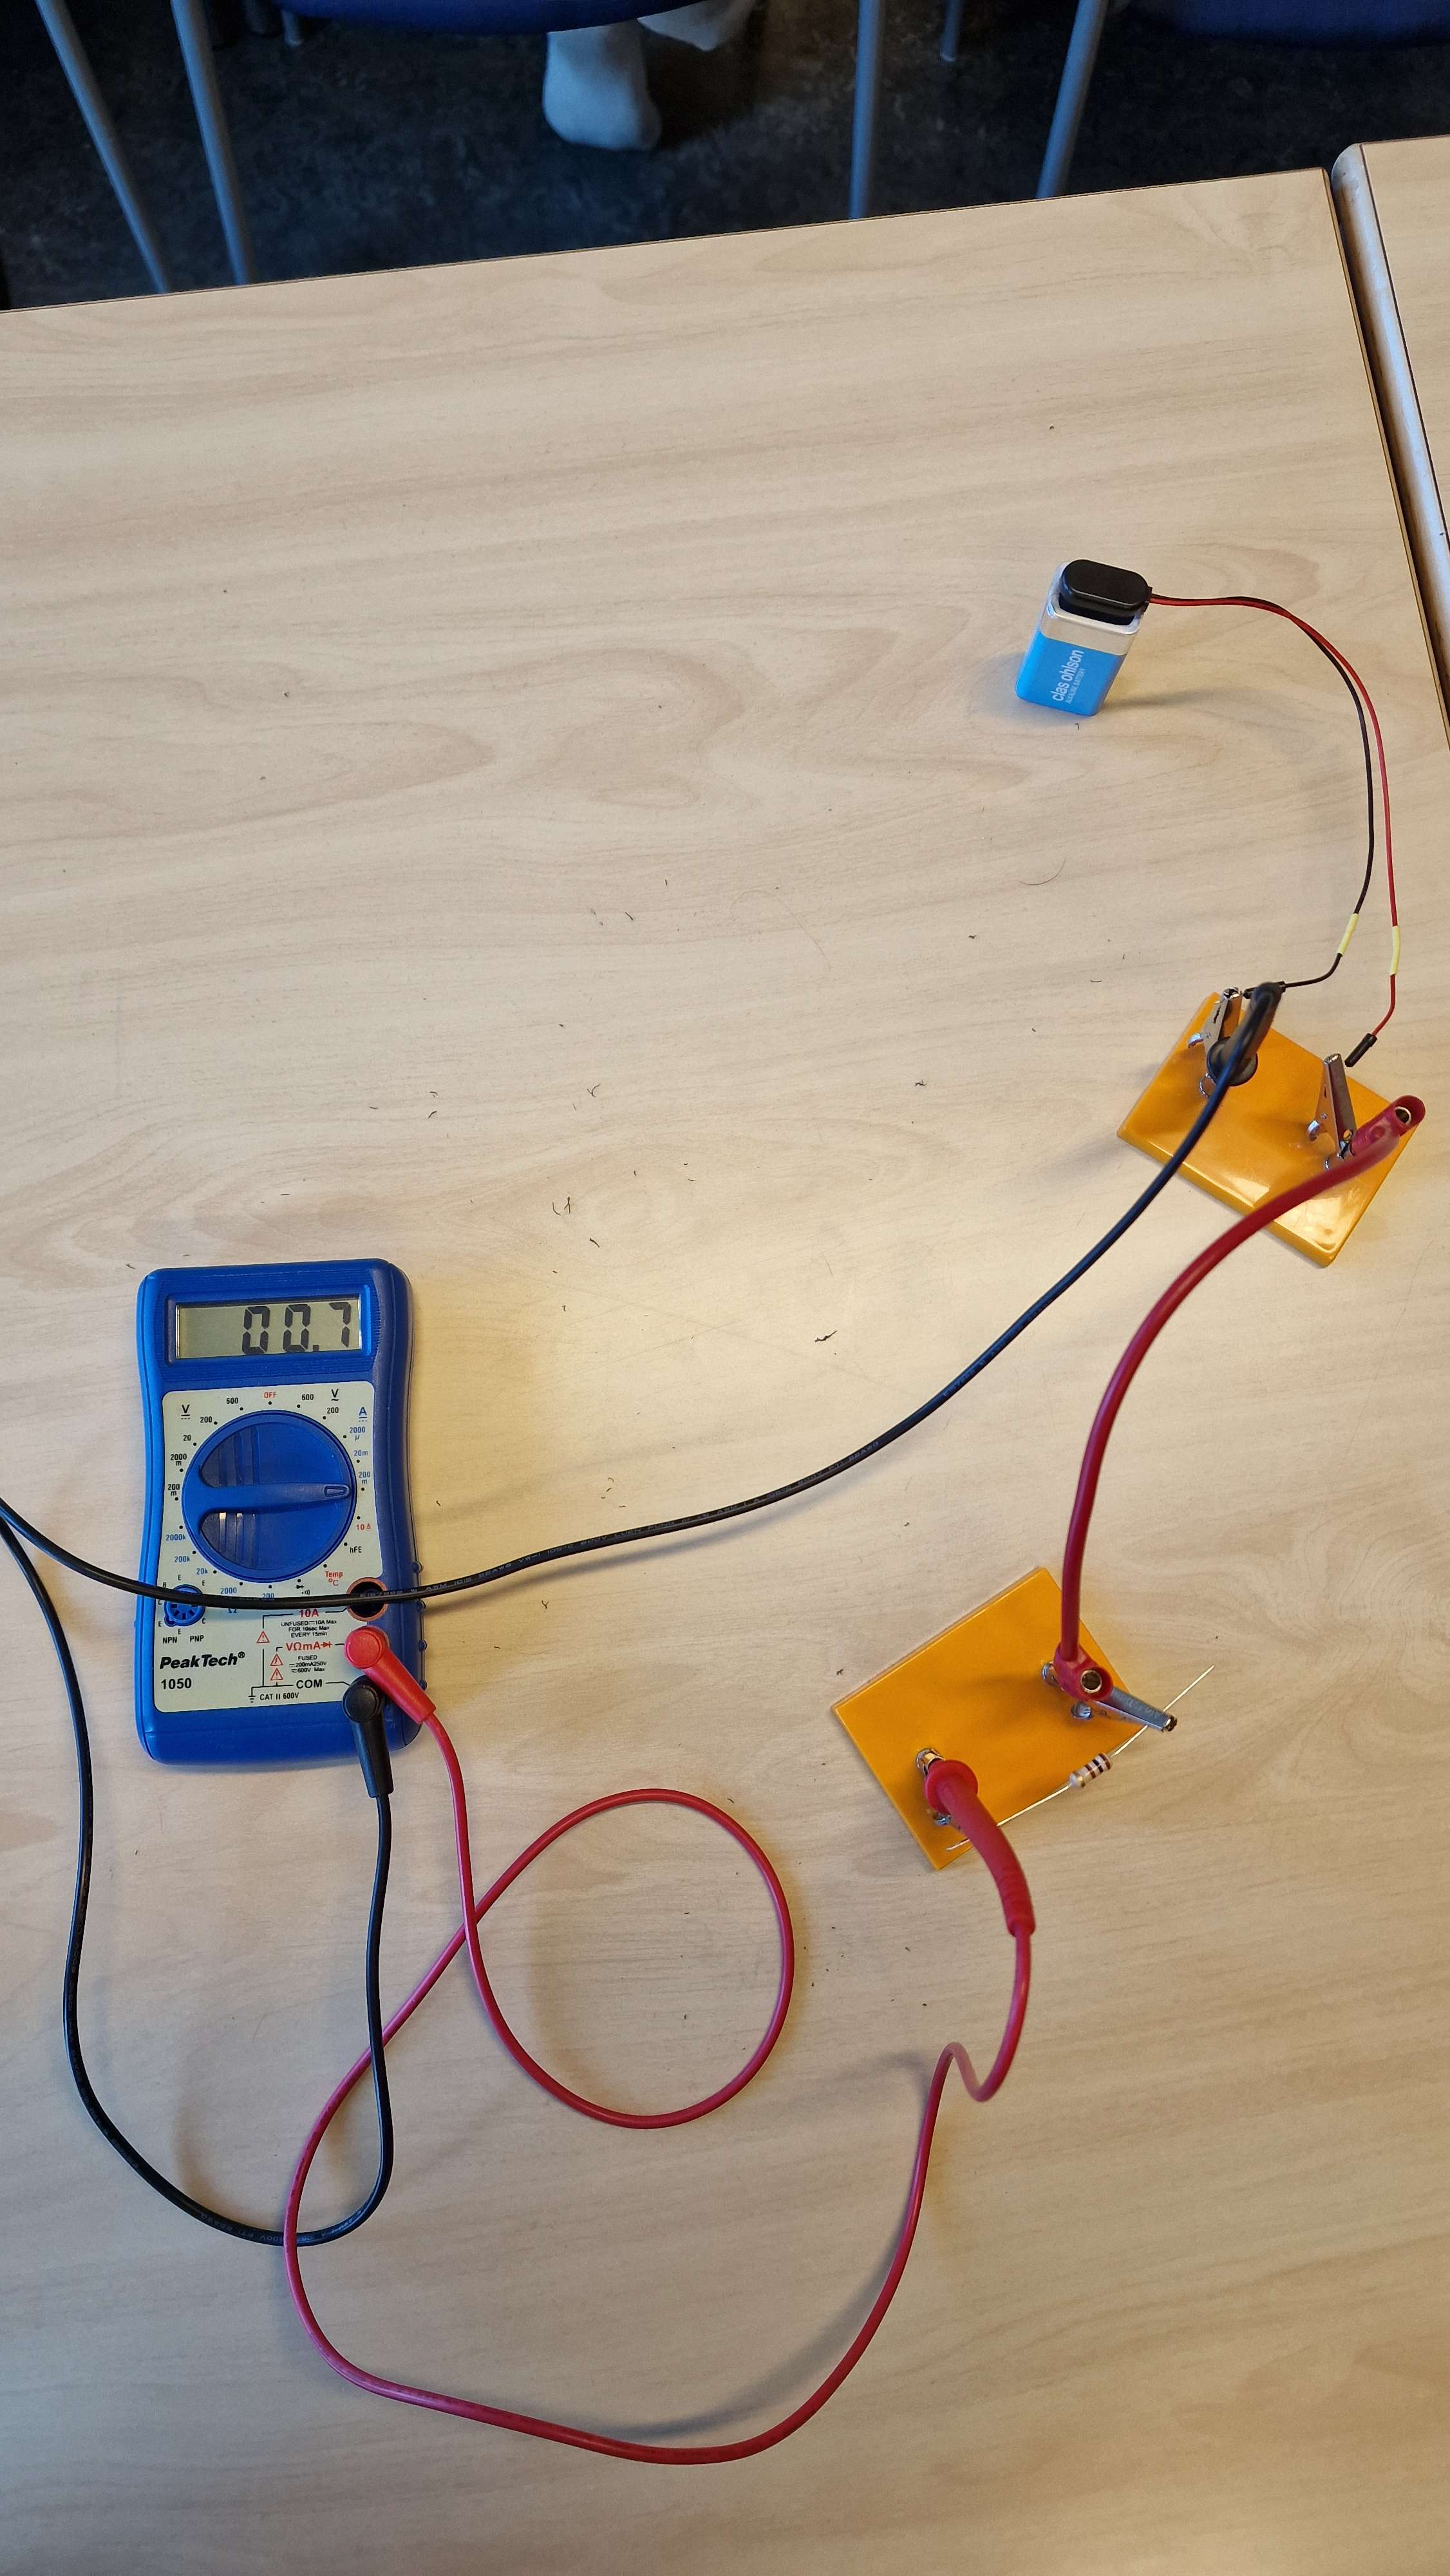
\includegraphics[width=0.3\textwidth]{images/1Volt.jpg}
        \item Sätt först multimetern till 20V och skriv ner resultatet.
        \\
        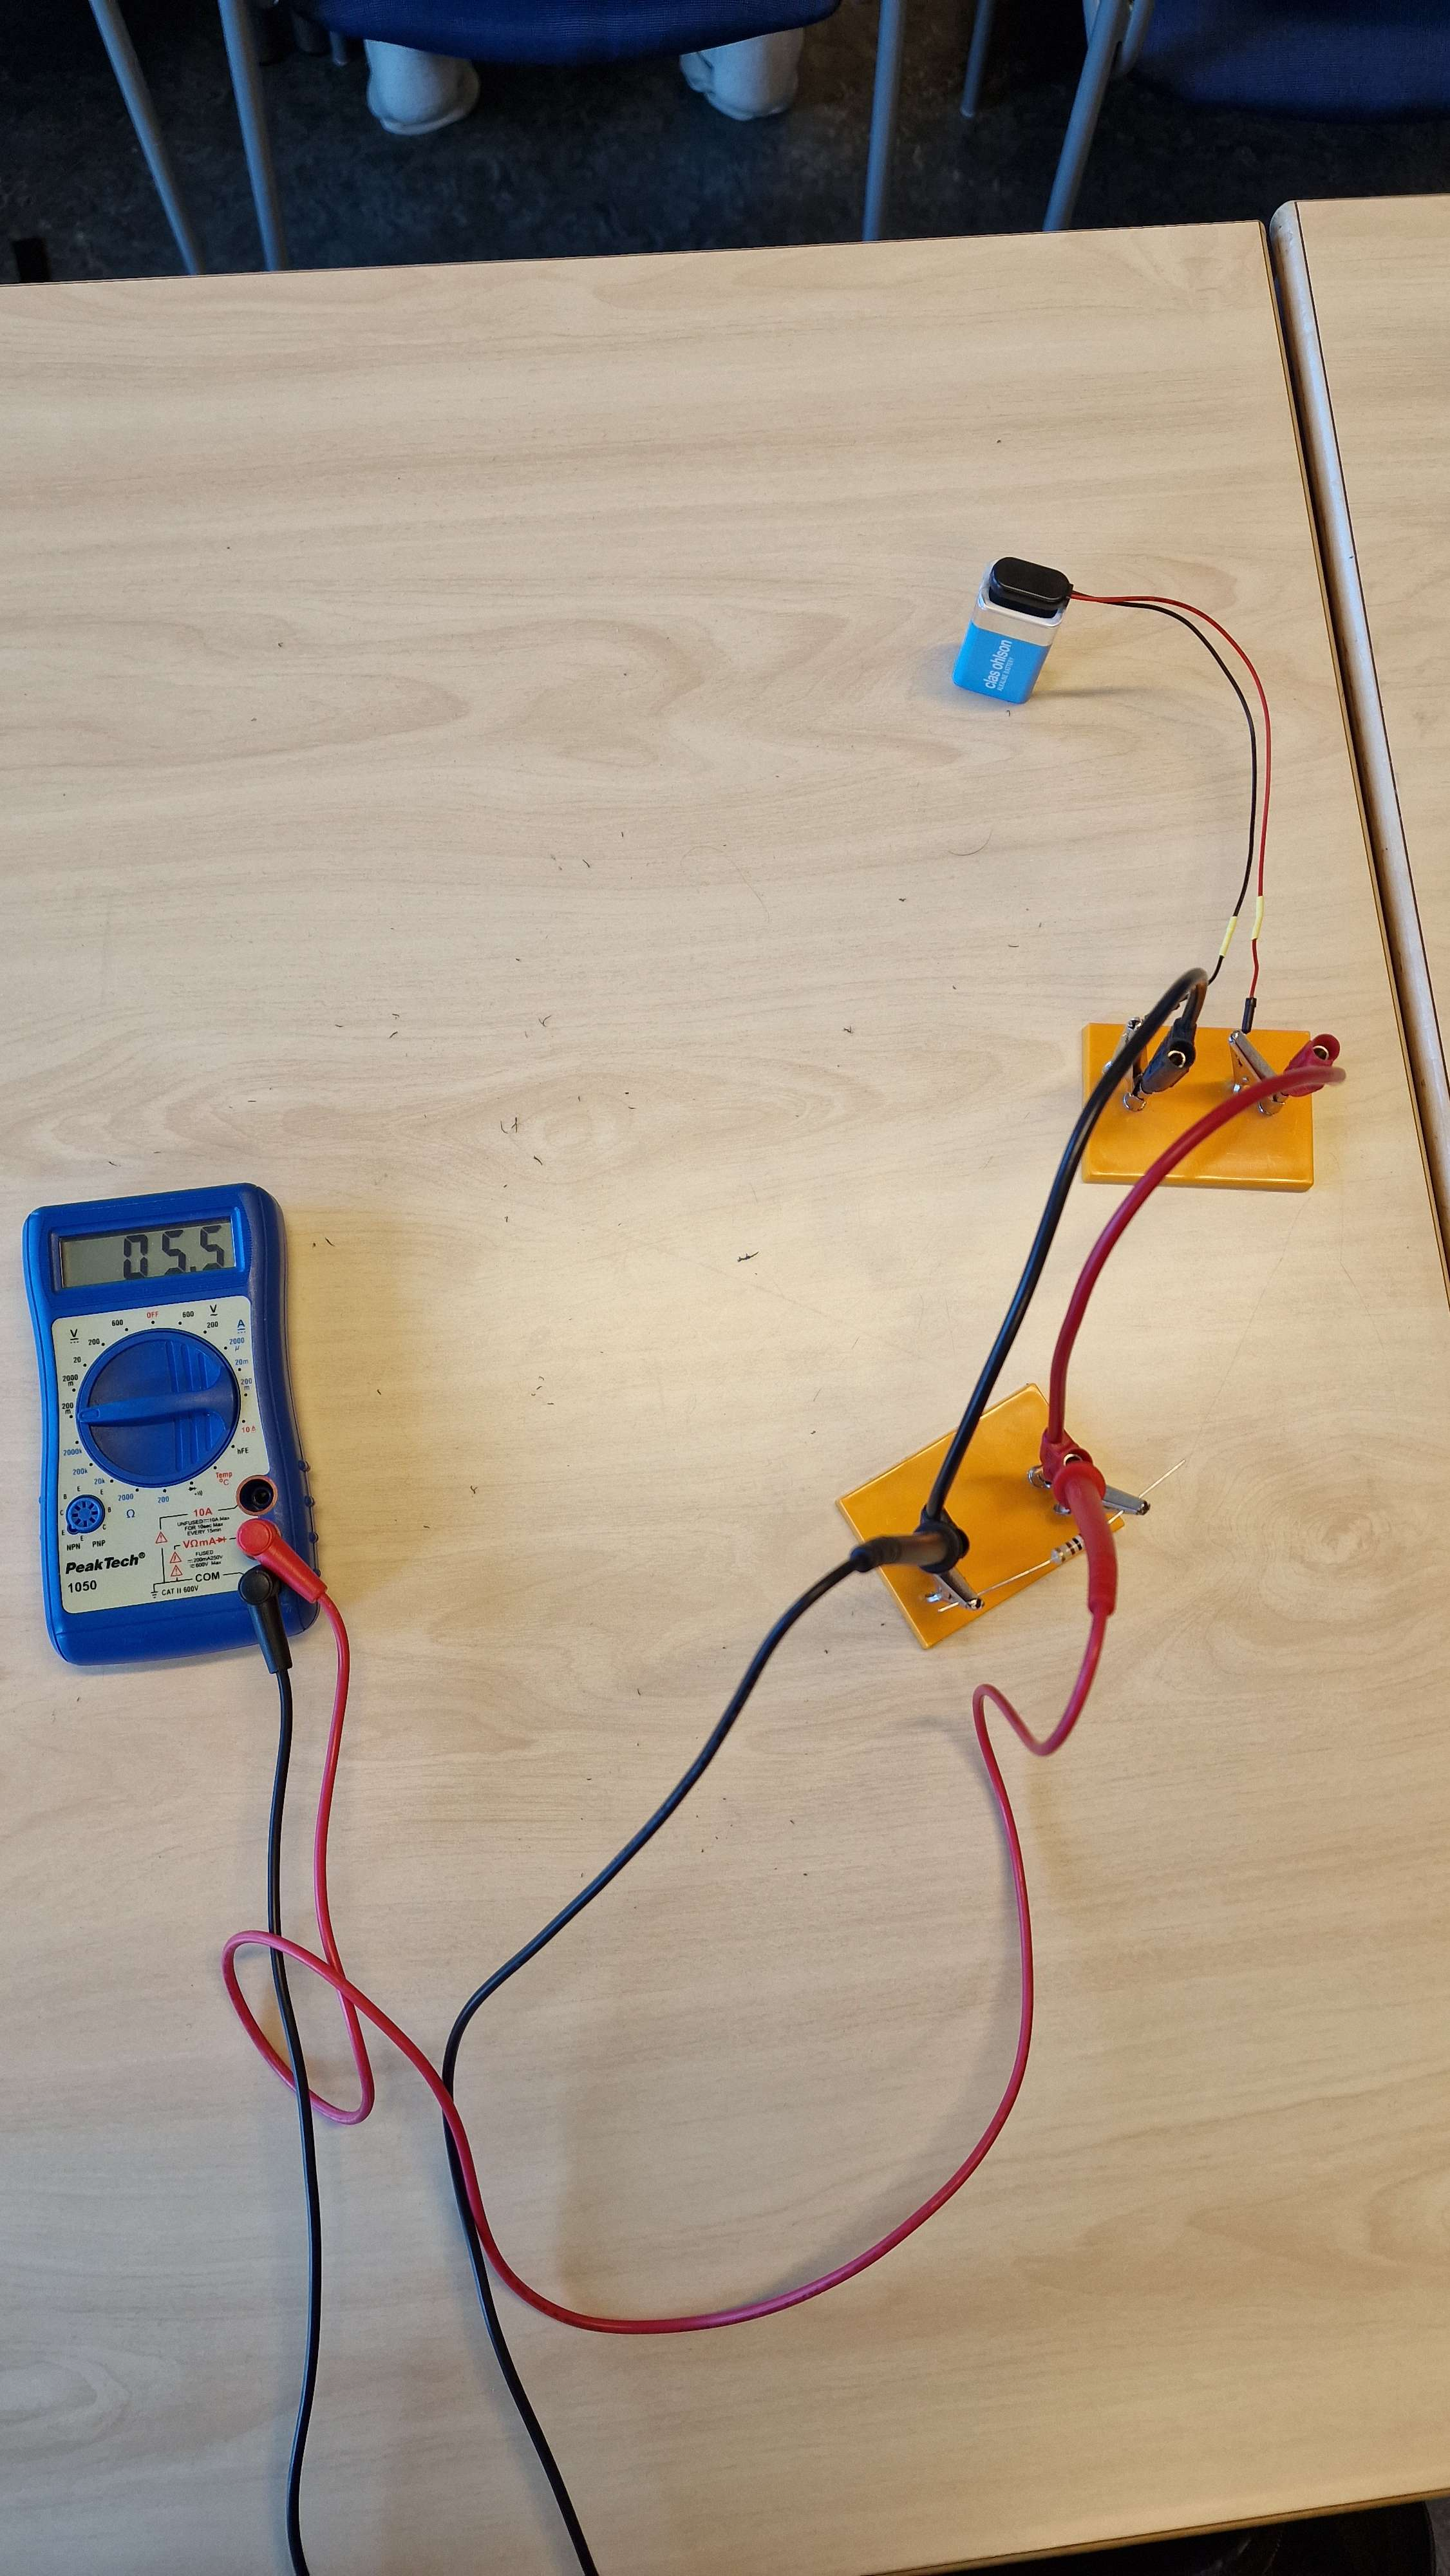
\includegraphics[width=0.3\textwidth]{images/1Ampere.jpg}
        \item sedan koppla multimetern igenom resistorn och sätt multimetern på 200mA, skriv sedan ner resultatet.
    \end{enumerate}

    \subsection{Resultat}
    De resultat vi fick var 0,03V och 0,0003A.

    \subsection{Analys}
    Om vi nu utgår från Ohms lag, U = RI, och omskriver den till, U/I = R. Om vi placerar in våra mätvärden så får vi att, 0.03/0.0003 = $100\Omega$, vilket då visar att resistansen bakom resistorn är $100\Omega$.

    \section{Del 2}
    \subsection{Metod}
    Målet med andra delen är att mäta Ström och Spänning i en seriekoppling.

    \begin{enumerate}
        \item Koppla ihop Batteriet med resistorn.
        \item koppla ännu en resistor i serie med det första.
        \item Koppla multimetern över resistorn.
        \\
        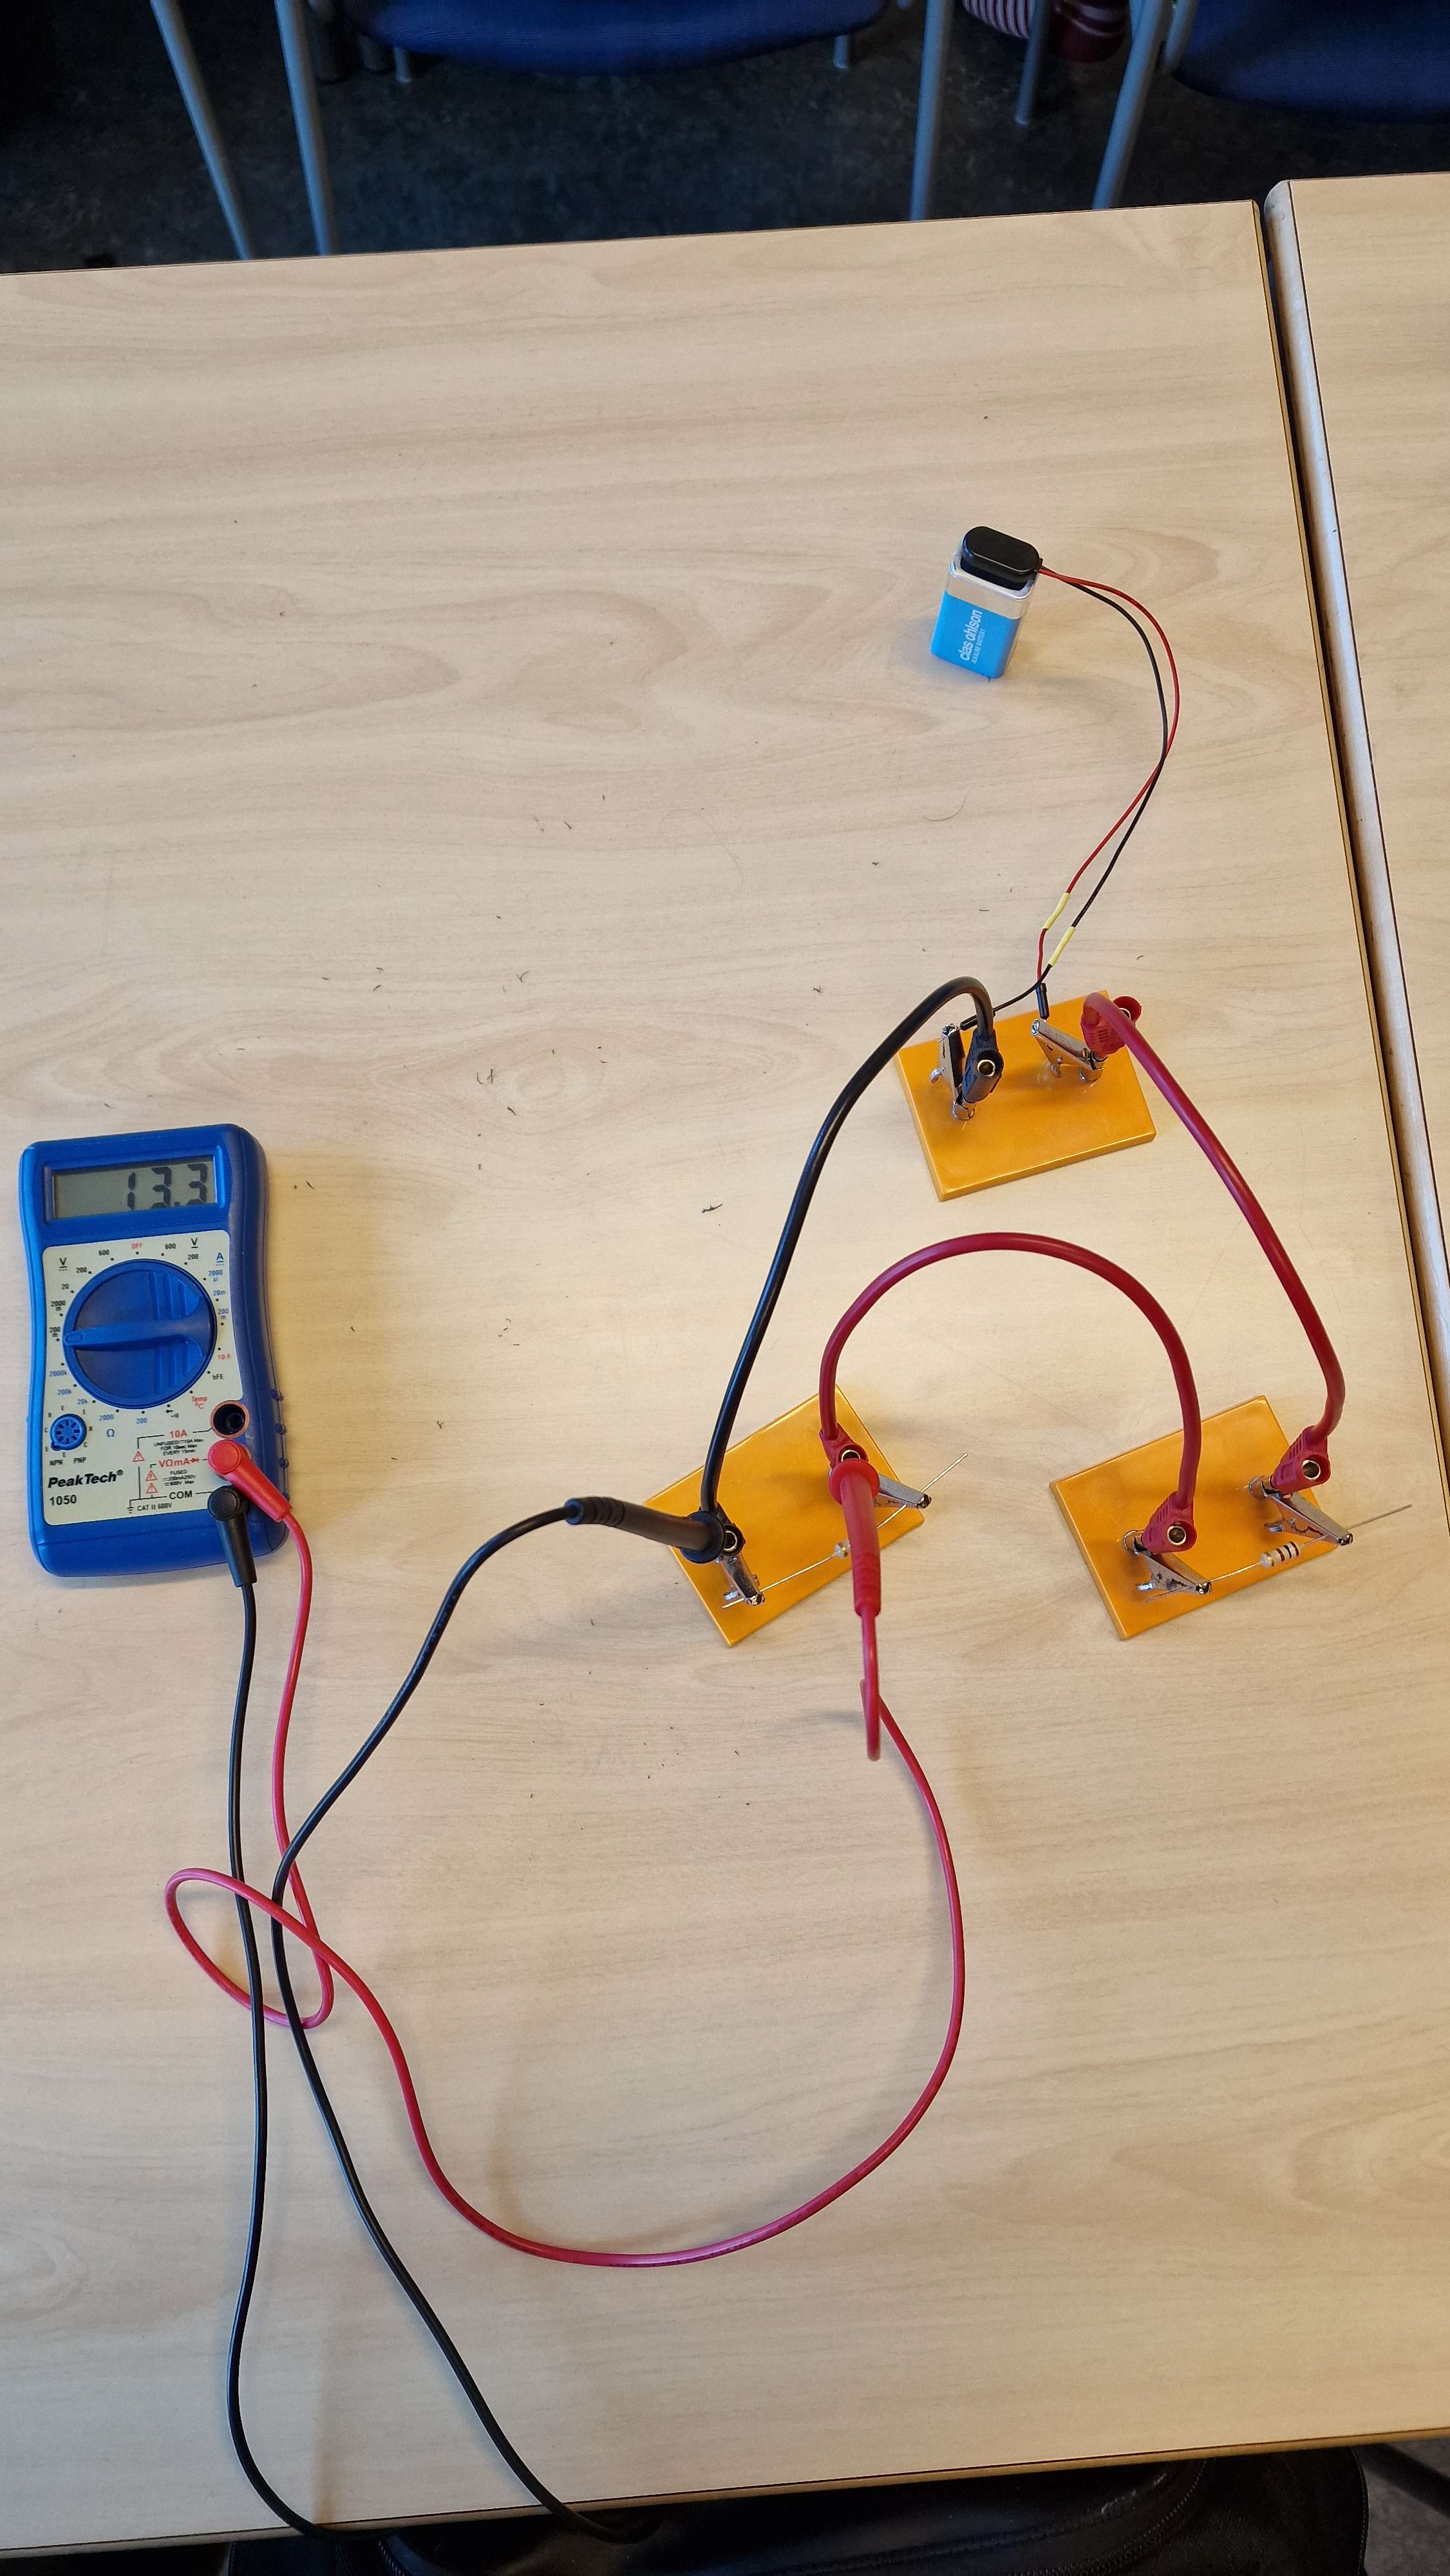
\includegraphics[width=0.3\textwidth]{images/2Volt.jpg}
        \item Sätt först multimetern till 20V och skriv ner resultatet.
        \\
        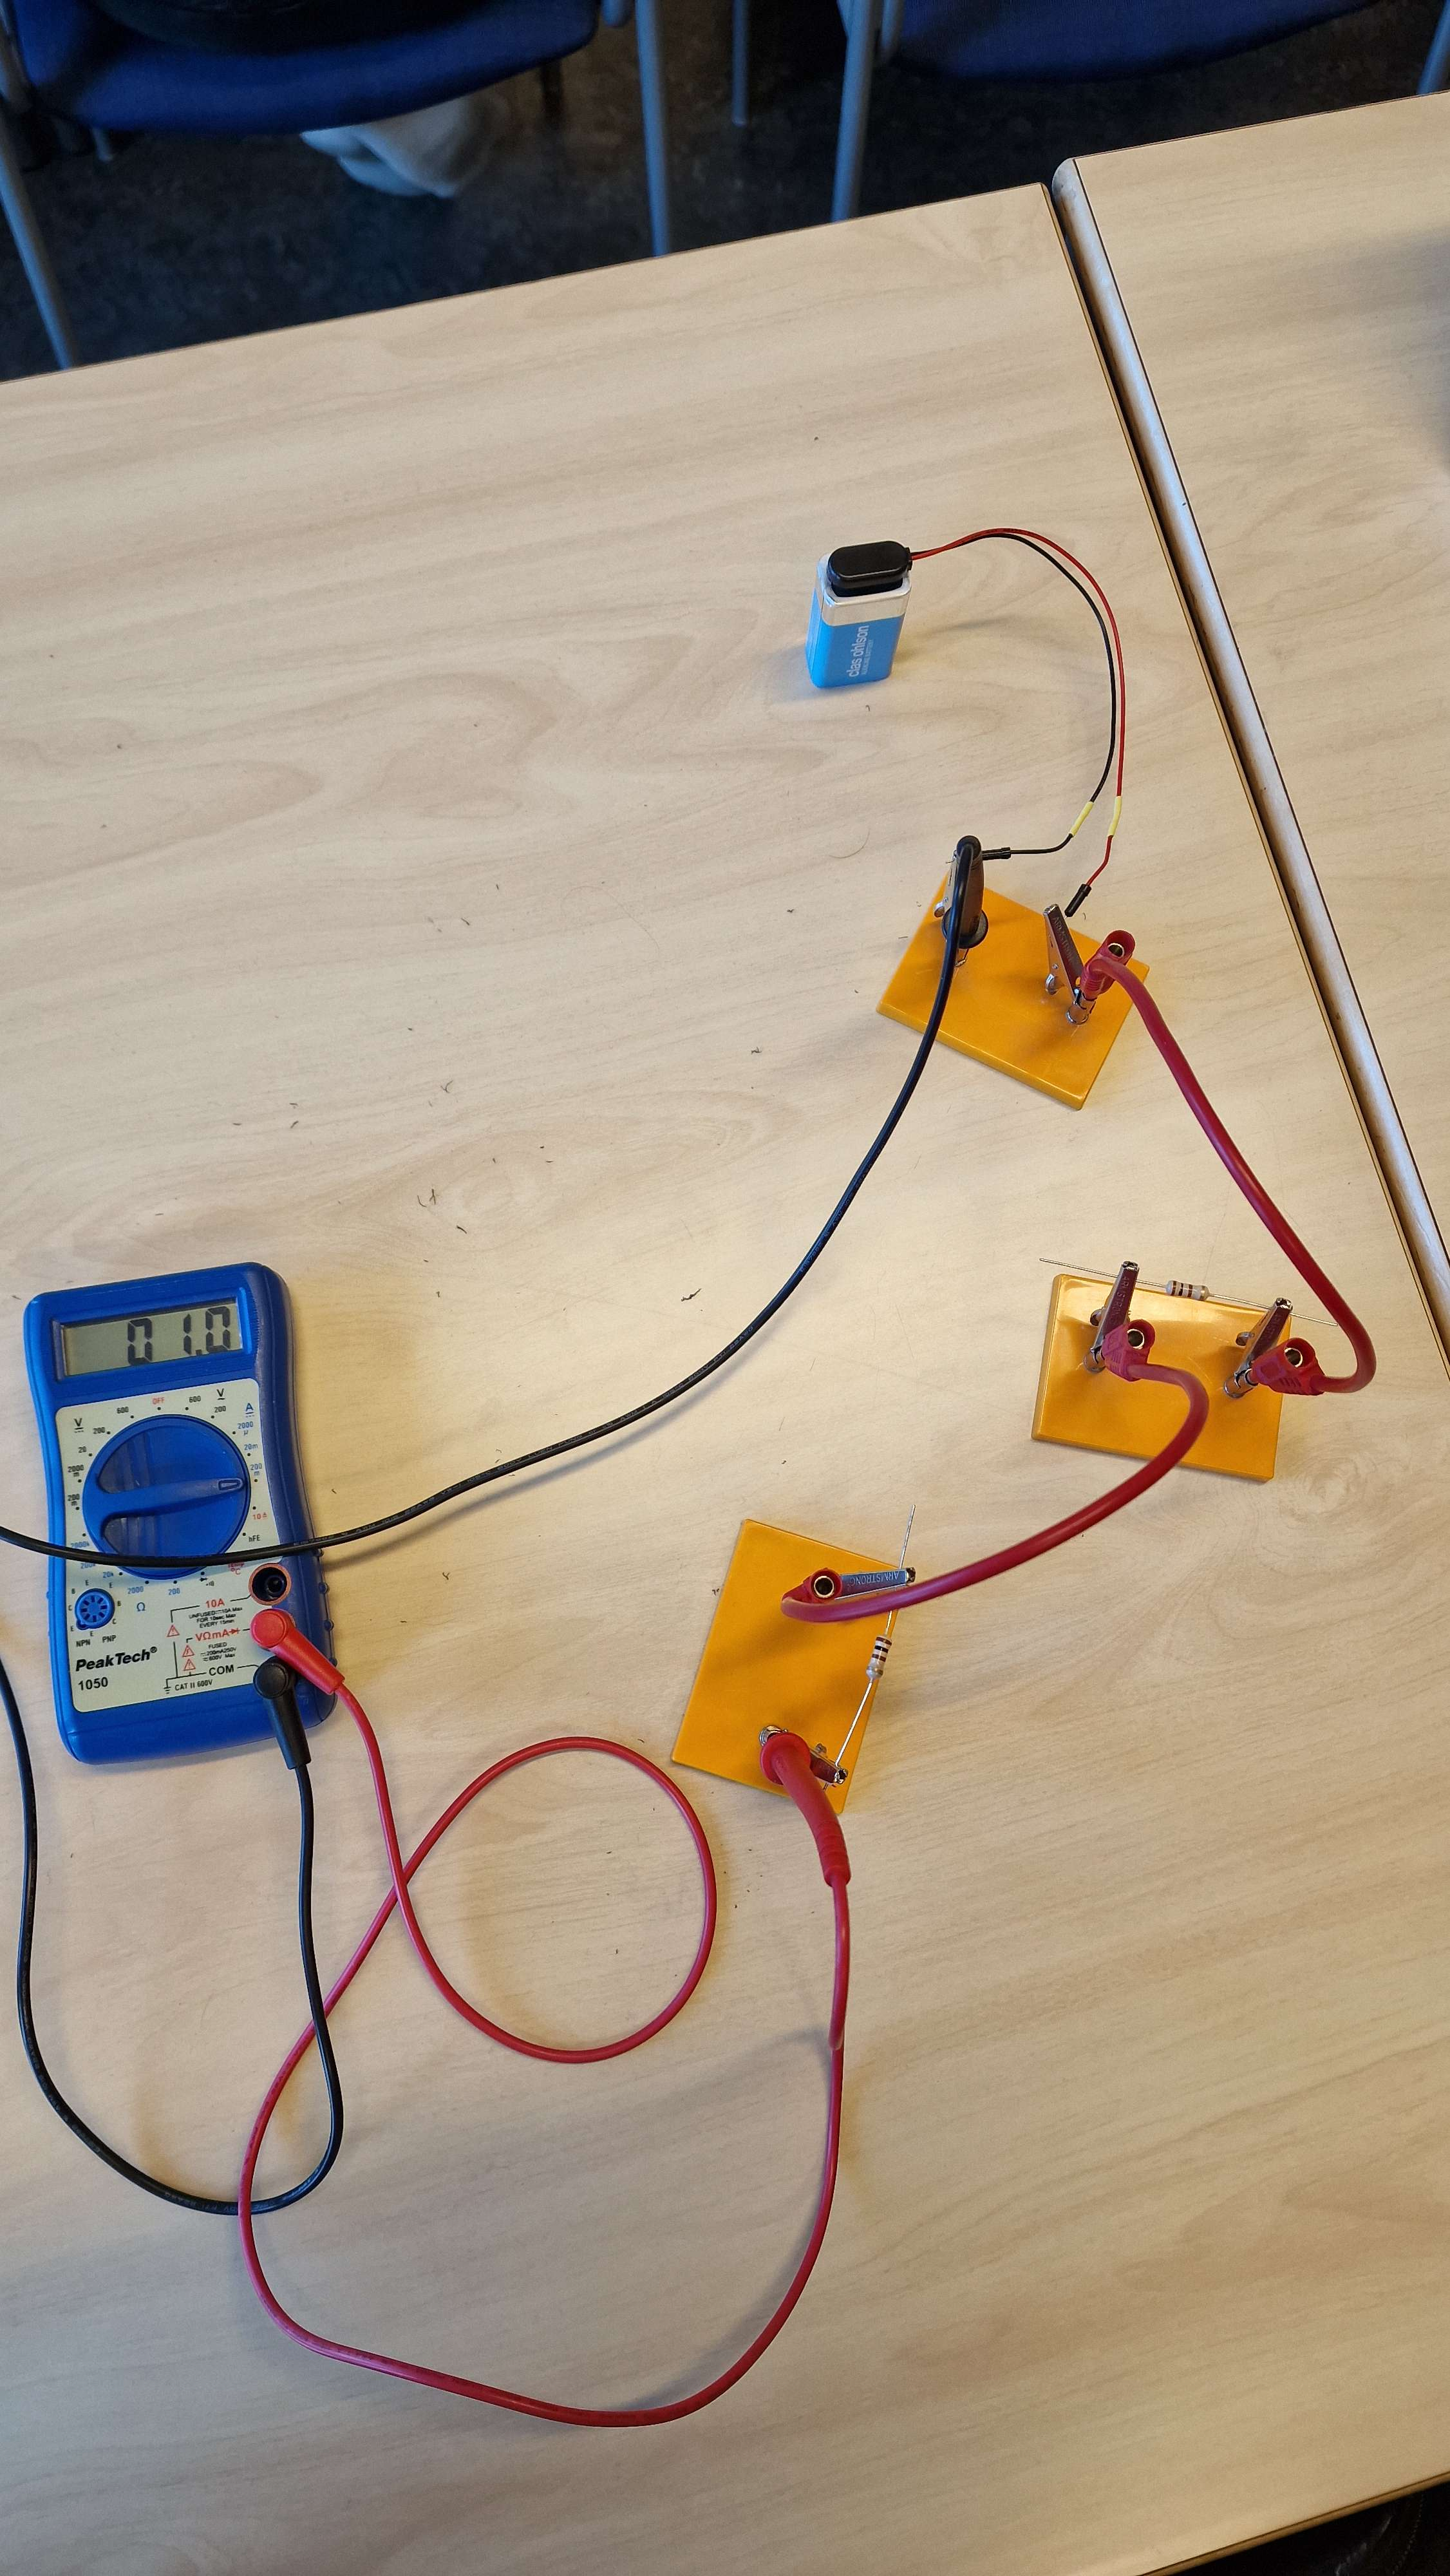
\includegraphics[width=0.3\textwidth]{images/2Ampere.jpg}
        \item sedan koppla multimetern genom en resistorn och sätt multimetern på 200mA, skriv sedan ner resultatet.
    \end{enumerate}

    \subsection{Resultat}
    De resultat vi fick var 0,015V och 0,0003A.

    \subsection{Analys}
    Med att det är en seriekoppling så måste vi lägga ihop resistanserna, R = R_1 + R_2.Vilket då ger oss, $100\Omega$ + $100\Omega$ = $200\Omega$.\\
    Med detta kan vi nu räkna ut vad vi borde få utifårn teorin, U = RI och U/R = I, dessa två då ger oss, 200*0.0003 = 0.06V och 0.03/200 = 0.00015A.

    \section{Del 3}
    \subsection{Metod}
    Målet med tredje delen är att måta Strömen och Spänningen i en parallelkoppling.

    \begin{enumerate}
        \item Koppla ihop Batteriet med resistorn.
        \item koppla ännu en resistor parralelt med den första resistorn.
        \item Koppla multimetern över resistorn den ena resistorn.
        \\
        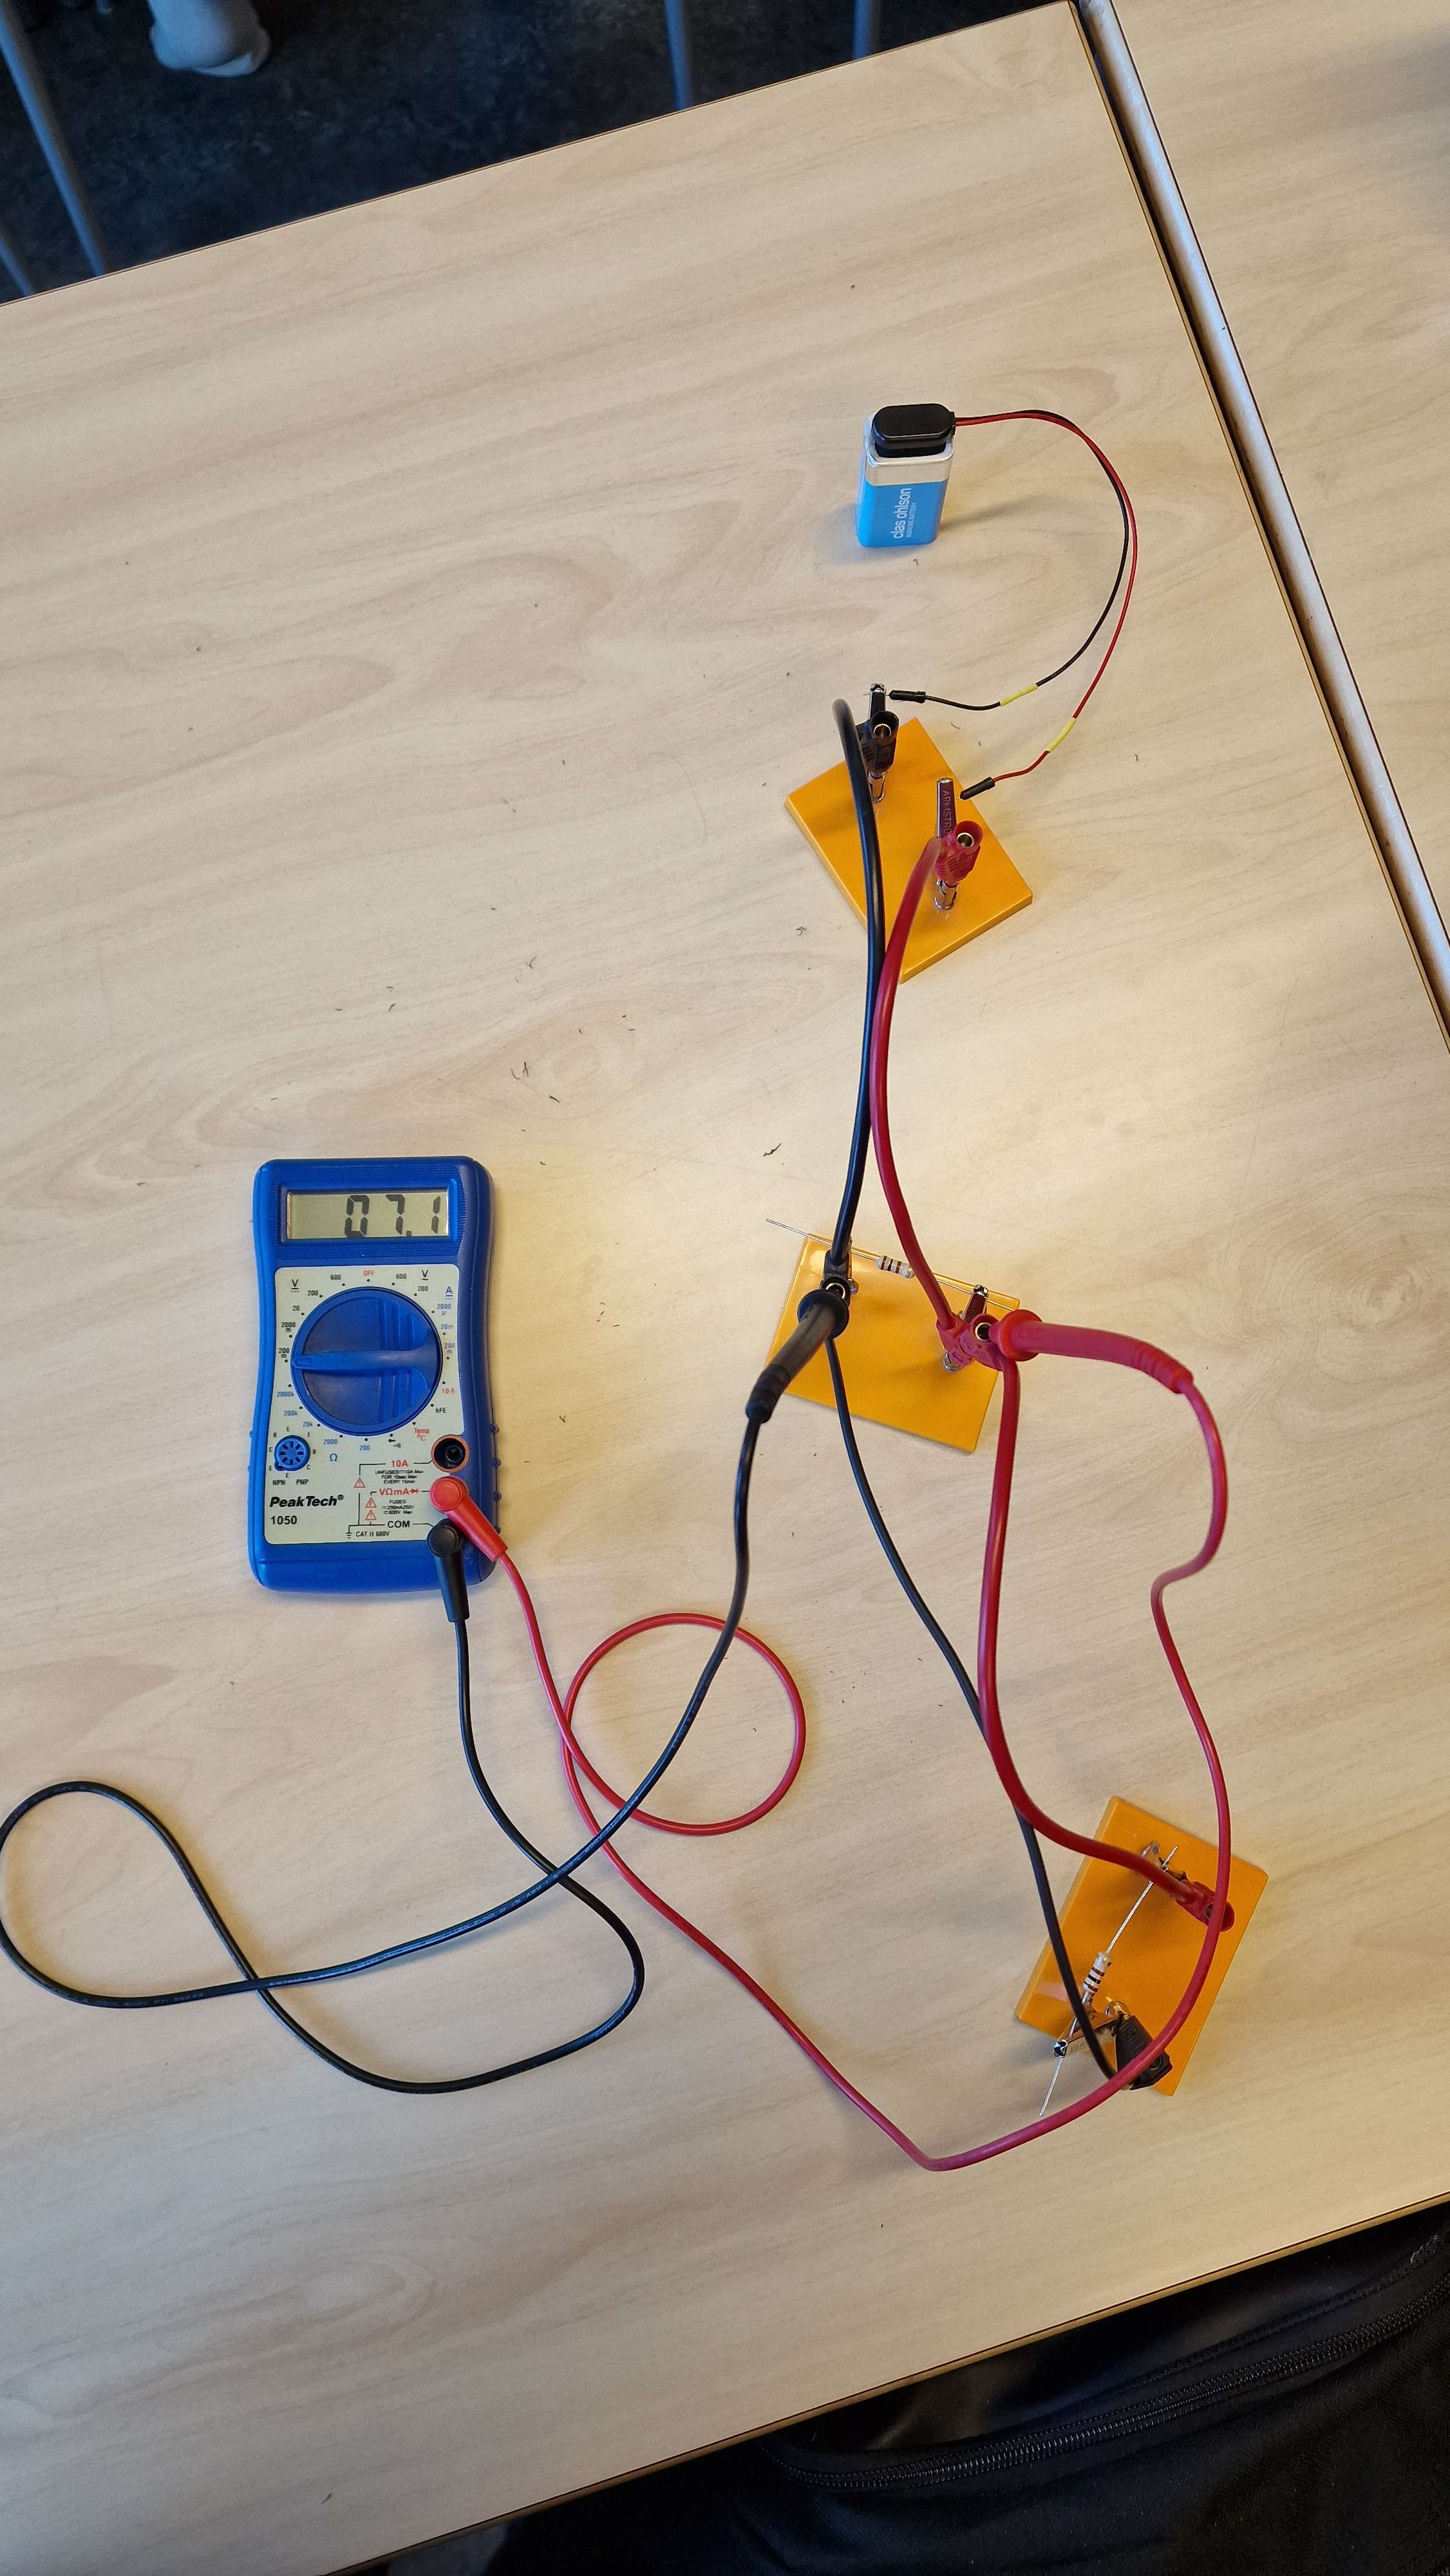
\includegraphics[width=0.3\textwidth]{images/3Volt.jpg}
        \item Sätt först multimetern till 20V och skriv ner resultatet.
        \\
        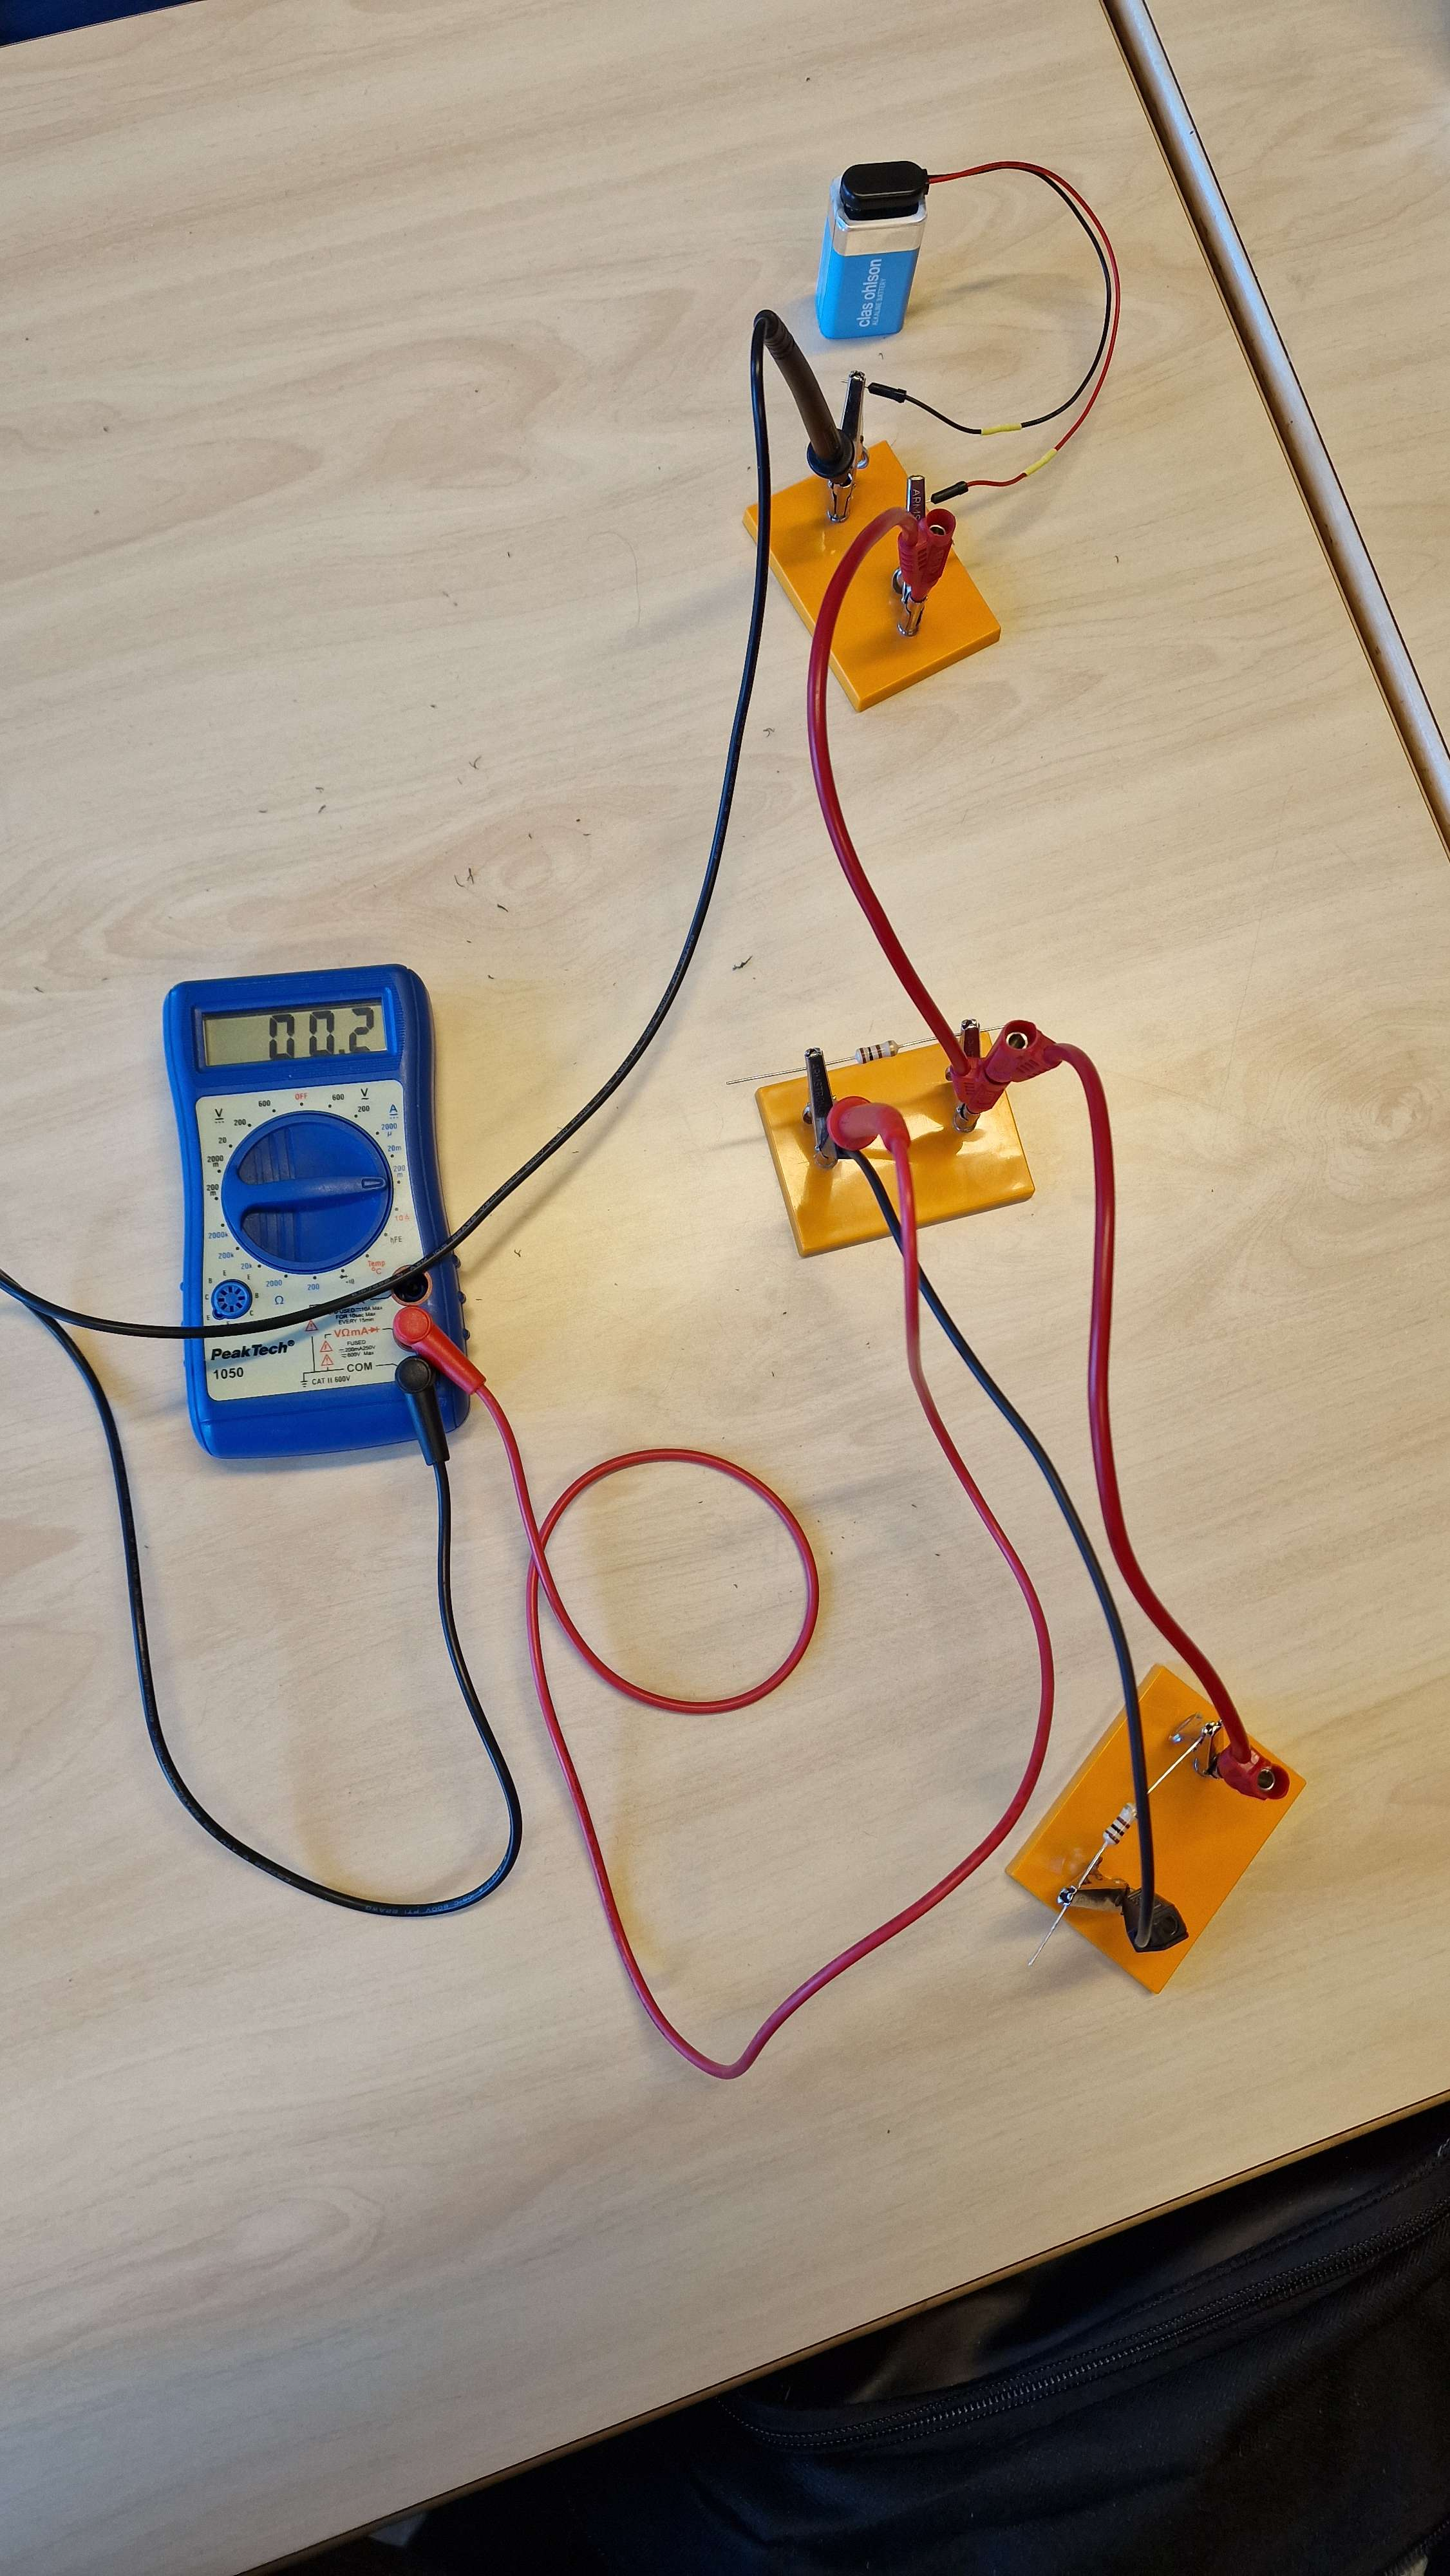
\includegraphics[width=0.3\textwidth]{images/3Ampere.jpg}
        \item sedan koppla multimetern genom en resistorn och sätt multimetern på 200mA, skriv sedan ner resultatet.
    \end{enumerate}

    \subsection{Resultat}
    De resultat vi fick var 0,03V och 0,0003A.

    \subsection{Analys}
    Med att det är en parallelkoplling måste vi lägga ihop resistanterna enlight det följande, $\frac{1}{R}$ = $\frac{1}{R_1}$ + $\frac{1}{R_2}$, vilket då ger oss, $\frac{1}{100\Omega}$ + $\frac{1}{100\Omega}$ = $50\Omega$.\\
    Med detta då kan vi räkna ut både Volten och Amperen med det följande, U = RI och $\frac{U}{R}$ = I, vilket då ger oss, 50*0.0003 = 0.015V och $\frac{0.03}{50}$ = 0.0006A.

    \section{Diskussion}
    Våra resultat i jämförelse med teorin är ej det samme, detta tyder då på att någonting inom våran laboration antingen inte stämde till eller så är det en fråga om fel avläsning.\\
    \\
    Om laborationen skulle göras om så skulle vi kunnat vara nogranare med både utförandet men också avläsandet och dokumentationen därmed.

\end{document}
